\vssub
\subsection{~Spectral partitioning} \label{sub:num_part}
\conthead{APL Wave / XWaves / IMEDS}{B. Tracy, C. Bunney}

The sea-states predicted by numerical wave models are often complex, due to the
presence of multiple wave trains formed as a result of both local wind action and
more distant storms. In order to better describe these local wind-sea and remote
swell components, without dealing with the full complexity of the model wave spectrum,
the spectrum can be partitioned into collections of spectral bins from which more
recognisable wave statistics (height, period, direction) can be derived. 

\noindent
Fig. \ref{fig:partitions} shows an example surface plot of an energy density
spectrum at one grid point at a specific time.  The amount of energy density
at each frequency-direction intersection is shown by this surface.  The
surface is divided into shaded areas or partitions representing energy from
sub-peaks within the spectrum.  Fig. \ref{fig:partitions} shows four
spectral partitions, an area of windsea and three swell trains.  The total
energy represented by this spectrum can be defined by bulk parameters, such as
the significant wave height $H_s$. The shaded areas, called partitions of the
spectrum, show spectral sub-features that give more information about this
grid point's energy situation.  \ws\ has point and field output options
available to provide quantitative descriptions of these individual spectral
partition such as partition wave height, peak period of partition (parabolic
fit), peak wavelength of partition, mean direction of partition, wind-sea
fraction of partition ($W$) using Eq.~(\ref{eq:wsf}), and the number of
partitions.  In the field output, these parameters correspond to spectral partitioned output fields 
\ref{out:first_part} through \ref{out:last_part} and can be found in
\para\ref{sub:outpars}.

Across the wave forecasting community, various methods of spectral partitioning
and definition of waves as sea or swell have been adopted. Two varieties of partitioning
are available from the W3PARTMD module.
\begin{enumerate}
  \item Topographic partitioning that groups spectral bins together into (multiple) 
        distinct wave systems.
  \item A simple frequency based cutoff that produces two partitions; one above
        and one below a cutoff frquency.
\end{enumerate}
The topographic partitioning methods in \ws\ are all based on a watershedding technique
using the original partitioning code implemented by B. Tracey (see below). These are
further categorised according to the method by which a partition is determined to be
either wind-sea or swell. The cutoff methods are varied dependent upon whether the
user chooses to use a set frequency (e.g. to delineate between high frequency sea waves 
and lower frequency swells) or allows the threshold to vary according to the
local wind speed and direction.

\subsubsection{Topographic partitioning method}

Since the two-dimensional spectrum in Fig.~\ref{fig:partitions} looks like a
topological surface, it is logical to apply an image processing partitioning
algorithm that treats the spectral surface like a topographical surface.  The
partitioning shown in Fig.~\ref{fig:partitions} is based on a digital image
processing watershed algorithm \citep{art:VS91} first prototyped by
\cite{pro:HJ04} for the analysis of ocean wave data. 
The US continental divide where everything to the east goes into the Atlantic
Ocean and everything to the west goes into the Pacific Ocean is a typical
example of a watershed line.  The oceans represent minima that determine the
watershed line.  If the spectral surface is inverted, the spectral peaks
become catchments and watershed lines or partition boundaries can be
determined using the \cite{art:VS91} algorithm.  Calculation of parameters for
each spectral partition can then be accomplished and wave system analysis as
described in \cite{art:HP01} can be applied.  \cite{pro:HJ04} and
\cite{tol:Vict06b} used a MATLAB code to apply the \cite{art:VS91}
algorithm\footnote{~Now available as XWaves from
http://www.WaveForceTechnologies.com, replacing the previous APL WAVES
package}.  This code has been transformed to an efficient FORTRAN routine for
use in \ws since version 3.11.  Coding follows the
\cite{art:VS91} paper but incorporates an efficient sort routine (O(n))
discussed in \cite{rep:TTH06}.

\begin{figure} \begin{center}
\epsfig{file=./num/partition1.eps,width=3.8in}
\caption{Surface plot of an energy density spectrum showing spectral
         partitions for windsea and three swell trains.  This is a snapshot of
         hindcasted conditions at Christmas Island (NOAA buoy 51028) at
         12:00~UTC on November 9, 2000.}
         \label{fig:partitions} \botline
\end{center}
\end{figure}

\subsubsection{Sea/swell assignment and partitioning method}

The second stage in the partitioning process is the assignment of individual
partitions to (wind-)sea and swell categories in point or field outputs. In the
default option for \ws\ these comprise a single wind-sea (partition 1) and a set
of swell components ordered by wave height. Selecting alternative partition methods
changes the categorisation as described below. 

The partitioning method is set in the MISC namelist in ww3\_grid.inp via the PTM parameter:
\begin{itemize}

 \item PTM=1: Wind sea and swells defined using topographic partitions and
   		  classified using a wind sea fraction cutoff (WWIII default scheme).
		  Outputs wind-sea plus swell 1,2,3 etc.

 \item PTM=2: Wind sea and swells defined using topographic partitions and
          spectral wave-age cutoff. Outputs wind-sea plus swell 1,2,3 etc.
		  
 \item PTM=3: Wave components defined using topographic partitions only. Outputs partitions
          ranked by wave height as partition 1,2,3 etc.

 \item PTM=4: Wind sea and swell defined using spectral wave-age cutoff. Outputs wind-sea and single swell partition.

 \item PTM=5: Wave components defined using a user defined frequency cutoff (PTFCUT).
        Outputs high frequency and low frequency partition.
\end{itemize}

In PTM1, topographic partitions for which the percentage of wind-sea energy exceeds a 
defined fraction are aggregated and assigned to the wind-sea component (e.g., the first
partition). The remaining partitions are assigned as swell components in order of 
decreasing wave height.

PTM2 works in a very similar way to PTM1, by first identifying a primary wind-sea component,
which is assigned as the first partition, then a number of swell (or secondary wind-sea) 
partitions are identified, as follows. A set of secondary spectral partitions is established 
using the topographic method, each partition is checked in turn, with any of their spectral 
bins influenced by the wind (based on a wave age criterion) being removed and assigned as 
separate, secondary wind-sea partitions. The latter are by default combined into a single 
partition, but may remain separate if the namelist parameter FLC is set to ".False.". Swell 
and secondary wind-sea partitions are then ordered by decreasing wave height. Operational 
forecasts made at the Met Office suggests that when PTM2 is run with the default single wind-sea 
partition, this provides a smoother spatial transition between partitions and a more direct link 
between the primary wind-sea component and wind speed than PTM1. Using the default method, the 
fraction of wind-sea for all partitions except the primary wind-sea partition should be close to 0.0.

PTM3 does not classify the topographic partitions into wind-sea or swell - it simply orders
them by wave height. This approach is useful for producing data for spectral reconstruction 
applications using a limited number of partitions (e.g. \cite{pro:BSP13}), where the 
classification of the partition as wind-sea or swell is less important than the proportion
of overall spectral energy each partition represents.

Methods 4 and 5 do not use the watershedding partitioning method, but adopt
a simpler frequency cutoff that produces just two partitions. PTM4 uses the
wave age criterion derived from the local wind speed to split the spectrum in
to a wind-sea and single swell partition. In this case  waves with a celerity greater
than the directional component of the local wind speed are considered to be
freely propogating swell (i.e. unforced by the wind). This is similar to the
method commonly used to generate wind-sea and swell from the WAM model.

PTM5 works in a similar fashion but applies a user defined static frequency
cutoff to split the spectrum into a low- and high-band partition. The cutoff
frequency is defined as PTFCUT in the MISC namelist and defaults to 0.1Hz.
This method is useful if you have a downstream application that defines swell
simply as those waves in a spectrum with period greater than a predefined
constant value. This is similar to the default partitioning method found in SWAN.

For methods PTM1, PTM2 and PTM4 the wind cutoff can be controlled by modifying
the WSM factor in the MISC namelist. This applies a constant multiplier to the 
wind speed and defaults to 1.0.

At present the outputs using methods PTM1 and PTM2 should be obtained using any of the \ws\
standard output processing tools. The full range of partitioning methods are available for
gridded outputs using the ww3\_ounf module, and the netCDF file(s) that are produced will
include the partitioning method used within the variable attributes.

Note that for methods PTM4 and PTM5, only two partitions will ever be created,
therefore the NOSWLL parameter (defined in the MISC namelist; default=5) will
be overriden with a value of 2. Similarly, the wind sea fraction cutoff
value WSCUT will be set to 0.0.

Regression test \emph{regtests/ww3\_tpt1.1} provides examples of each
partitioning method.
